\documentclass[a4paper, 10pt, conference]{ieeeconf}

\IEEEoverridecommandlockouts
\overrideIEEEmargins

\usepackage{graphics} % for pdf, bitmapped graphics files
\usepackage{epsfig} % for postscript graphics files
\usepackage{mathptmx} % assumes new font selection scheme installed
\usepackage{times} % assumes new font selection scheme installed
\usepackage{amsmath} % assumes amsmath package installed
\usepackage{amssymb}  % assumes amsmath package installed
\usepackage{hyperref}
\usepackage{listings}

\usepackage[T1]{fontenc}
\usepackage[utf8]{inputenc}
\usepackage[brazil]{babel}
\usepackage{etoolbox}
\patchcmd{\abstract}{Abstract}{Resumo}{}{}
\patchcmd{\thebibliography}{References}{Referências}{}{}

\title{\LARGE \bf Uma linguagem de programação para processamento de imagens}

\author{Henrique Miyamoto e Thiago Benites}


\begin{document}
\maketitle
\thispagestyle{empty}
\pagestyle{empty}

%\begin{abstract}

%Escreva aqui o resumo (abstract).

%\end{abstract}

\section{Contextualização}

%Um breve texto introdutório explicando do que se trata o documento, em uma linguagem que poderia ser entendida por qualquer pessoa que entenda programação (ou seja: referências diretas à disciplina não são desejáveis).

Apresentamos uma linguagem de programação voltada para o processamento de imagens e implementada com o analisador léxico Flex \cite{flex} e o compilador de compilador GNU Bison \cite{bison}, utilizando funcionalidades da biblioteca FreeImage \cite{freeimage}. As funcionalidades que ela é capaz de executar, assim como as respectivas sintaxes são apresentadas na Tabela \ref{tabela1}.

\begin{table}[h]
	\centering
	\caption{Funcionalidades e sintaxe da linguagem de progrmação}
	\label{tabela1}
	\begin{tabular}{|c|c|}
		\hline
		Funcionalidade        & Sintaxe                                                                                                                \\ \hline
		Salvar uma imagem     & \texttt{destino.jpg = origem.jpg}                                                                                    \\ \hline
		Alterar brilho        & \begin{tabular}[c]{@{}c@{}}\texttt{destino.jpg = origem.jpg * float}\\ \texttt{destino.jpg = origem.jpg / float}\end{tabular} \\ \hline
		Detectar valor máximo & \texttt{[origem.jpg]}                                                                                            \\ \hline
	\end{tabular}
\end{table}

Nos casos de salvar uma imagem e de alterar seu brilho, é feita uma cópia do arquivo original. O valor de cada pixel foi calculado como a intensidade na conversão do espaço RGB para o HSI, i.e., tomamos $I=\frac{1}{3}(R+G+B)$ \cite{rgb}.

\section{Demonstração}

%Entradas e saídas que demonstram as funcionalidades implementadas.

\begin{figure}[h]
	\centering
	\label{opato}
	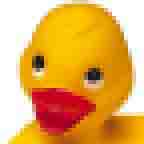
\includegraphics[width=5cm]{Figuras/pato}
	\caption{Relação da Teoria da Informação com outras áreas.}
\end{figure}

Para demonstração das funcionalidades, tomemos por base a imagem apresentada em sua forma original na Figura \ref{opato}.

\begin{lstlisting}[language=C, basicstyle=\footnotesize, frame=single]
int main(){
coloque_o_seu(codigo, aqui);
}
\end{lstlisting}

\section{Análise}

Comparando a idéia de usar os comandos específicos da linguagem para aplicar brilho com uma aplicação equivalente, usando alguma biblioteca de linguagem de propósito geral (por exemplo, `OpenCV`). A análise deve se basear em dados reais, e mostrar todos os dados sobre os quais ela se baseia (exemplos de código, citações bibliográficas ou outros dados que o grupo considere relevantes).

\begin{thebibliography}{99}

\bibitem{flex} GitHub. The Fast Lexycal Analyzer. Disponível em: \url{https://github.com/westes/flex}. Acesso em: 9 set. 2017. 

\bibitem{bison} GNU Bison. Disponível em: \url{http://www.gnu.org/software/bison/}. Acesso em: 9 set. 2017.

\bibitem{freeimage} FreeImage. Disponível em: \url{http://freeimage.sourceforge.net/}. Acesso em: 10 set. 2017.

\bibitem{rgb} Wikipedia. RGB color model. Disponível em: \url{https://en.wikipedia.org/wiki/RGB_color_model}. Acesso em: 10 set. 2017.

\end{thebibliography}

\end{document}